\section{Original-Code CryoLike Scoring on Experimental Particles}
\label{sec:cryolikecomparison}
We execute the original CryoLike CPU comparison routines
\citep{cryolike2025}, pinned to author commit
\texttt{a413ffd} (full hash retained in the protocol). The convenience file runner
requires CUDA; the original lower-level Fourier--Bessel comparator and
integrated-score kernels support CPU execution. A local adapter handles array
axes and physical units; independent asymmetric direct Fourier sums check both
image and volume conventions. No author scoring code is modified.

From the previously examined prediction cohort, select one particle per source
exposure, ordered by exposure string, up to 128: the resulting counts are
115, 71 and 128 for 10028, 10049 and 10076. Compare the averaged locked half maps
for Gaussian, voxel and stock neural reconstructions, plus the deposited EMDB
map on the same field. The learned maps used supplied training poses; scoring
does not use deposited poses or shifts. Known CTFs remain an external input.
This is exploratory reuse of observations, not a new frozen validation cohort.

Use Fourier radius twelve, polar radial step 0.25 in the author's units,
128 in-plane angles and 25 translations spanning $\pm2$ downsampled pixels per
axis. Execute both 0.4 and 0.2 radian viewing grids, containing 173 and 470
templates. Retain the author's image centering and normalization, template
DC-mask subtraction and polar normalization. The score is therefore not a
normalized raw-pixel predictive density for the preceding e-value construction.
All 24 cases complete; total runtime is 1,219 seconds under concurrent Mac load,
with 1.51 GB peak process memory. This is not a fine-resolution CUDA benchmark.

For each grid and geometry, compare each non-neural map with the neural map
using both maximum searched correlation and integrated log score. Retain all
36 contrasts. The declared descriptive uncertainty calculation uses 20,000
paired exposure bootstrap draws and percentile Bonferroni intervals within
each metric's eighteen-contrast family. These are bootstrap approximations,
not exact familywise guarantees or experimental density coverage.

\begin{figure*}[t]
\centering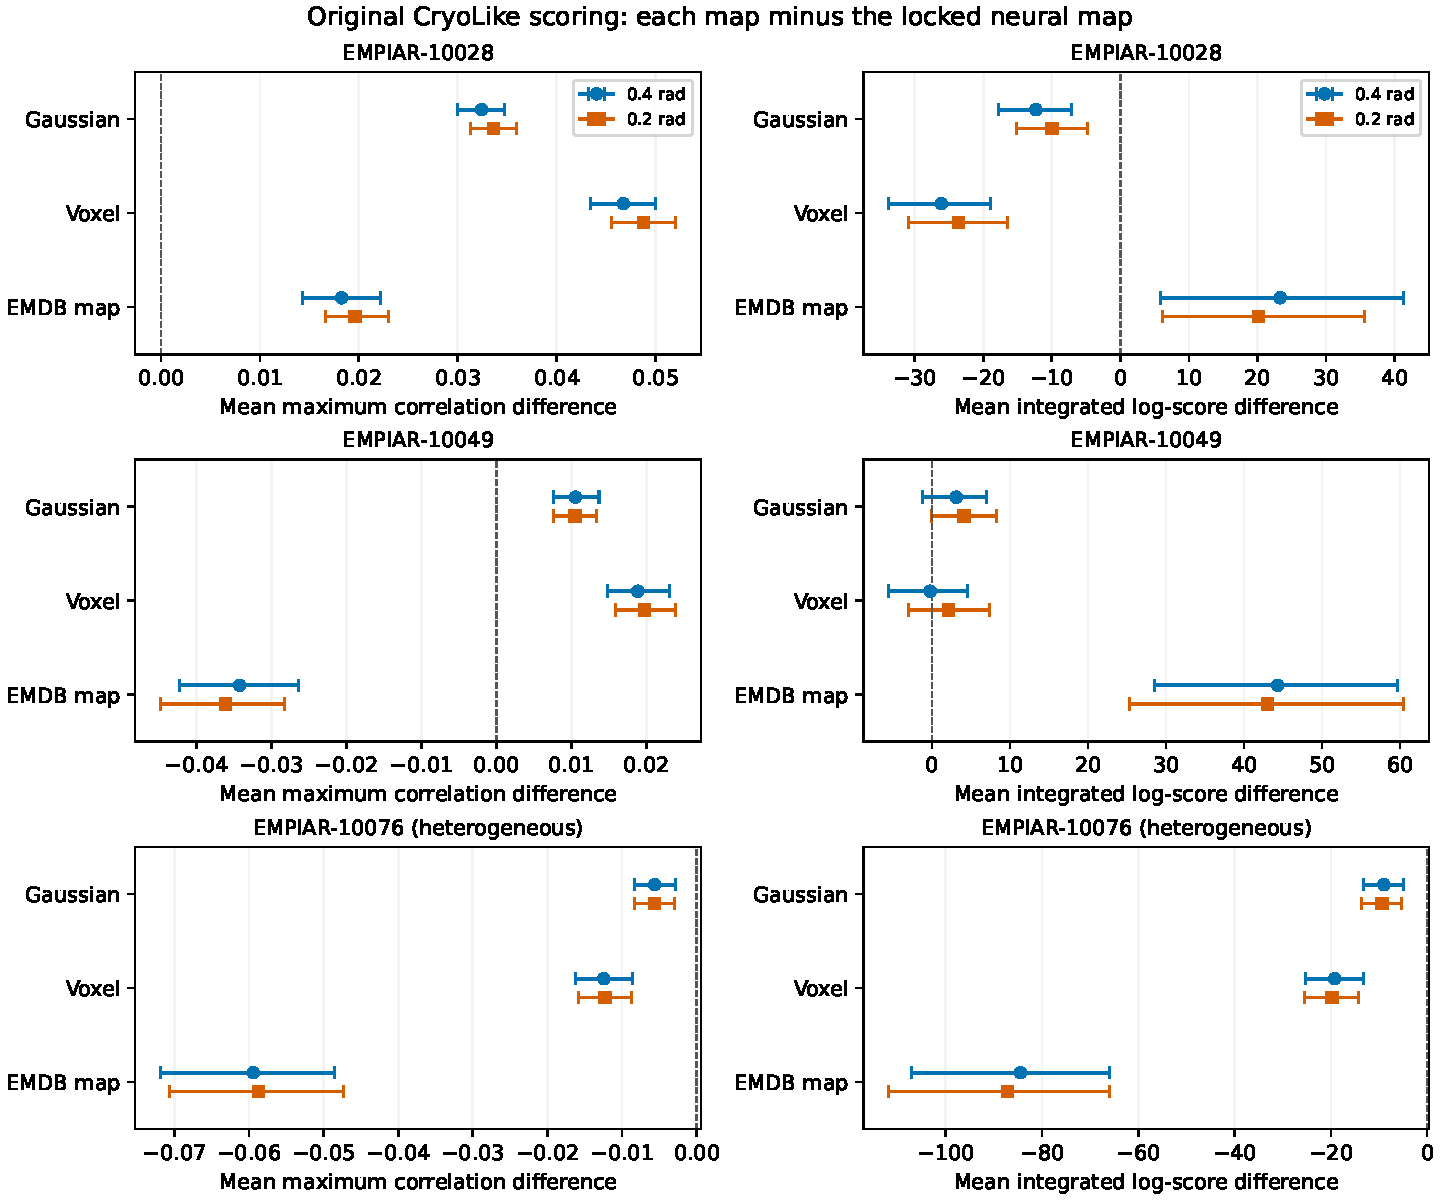
\includegraphics[width=.92\textwidth]{figures/cryolike-comparison.pdf}
\caption{All original-code CryoLike comparisons. Points show each map's mean
score minus the locked neural map's score; bars are the declared paired
bootstrap intervals with an eighteen-contrast Bonferroni adjustment per metric.
Both viewing grids are retained. Positive values favor the indicated map for
that score only. Maximum correlation and integrated score rank some maps
differently. These reused experimental exposures do not provide density truth
or validate the proposed continuous likelihood test.}
\label{fig:cryolikescoring}
\end{figure*}

Both grids give the same qualitative correlation ordering: Gaussian and voxel
exceed neural on 10028/10049 and fall below it on 10076, with the corresponding
family intervals excluding zero. Integrated log score instead favors neural
over both learned alternatives on 10028/10076; on 10049 all four intervals
include zero. The EMDB map's integrated score exceeds neural on 10028/10049
and falls below it on heterogeneous 10076, whereas its maximum correlation is
below neural on both 10049 and 10076. All these comparisons appear in
Figure~\ref{fig:cryolikescoring}. The differing metrics cannot establish a single
accuracy winner. The deposited maps are approximate, partly dependent
comparison structures, and these scoring outcomes do not demonstrate calibrated
uncertainty or a matched-power advantage for our method.
